\maketitle
\tableofcontents
\newpage

\section{Первое задание}

\paragraph{Текст задания} ~\\
(а)Представить слагаемые и результат в виде нормализованного числа с плавающей точкой двойной точ-ности: $(-1)^{s}(2^{e-1023})(1.f)$, где $1.f$ записанов двоичном виде.(б) Если результат неточный (не умещается целиком в мантиссе), то указать относительную погрешность ошибки. Исходные данные в десятичной системе счисления.

 \[ -1593.5859375 \cdot 2^{128} + 1619.09765625 \cdot 2^{141}\]

\paragraph{Решение} ~\\
Для начала разберемся с первым числом $-1593.5859375 \cdot 2^{128}$:
\begin{align*}
 %первое выражение
  -1593.5859375_{10}& = 11000111001.1001011_{2} = 1.10001110011001011_{2} \cdot 2^{10} \\[1mm]
%второе выражение
  -1593.5859375_{10} \cdot 2^{128}& = (-1)^{1}(2^{1161-1023}) \cdot 1.10001110011001011
\end{align*}
$s = 1$, $e = 1023+128+10 = 1161$, $f = 1000111001100101\underbrace{0\ldots0_{\text{35 нулей}}}$\\[1em]
Теперь нормализуем $1619.09765625 \cdot 2^{141}$:
\begin{align*}
%первое выражение
  1619.09765625_{10}& = 11001010011.00011001_{2} = 1.100101001100011001_{2} \cdot 2^{10} \\[1mm]
%второе выражение
  1619.09765625 \cdot 2^{141}& = (-1)^{0}(2^{1174-1023})(1.100101001100011001)
\end{align*}
$s = 0$, $e = 1023 + 141 + 10 = 1174$, $f = 100101001100011001\underbrace{0\ldots0_{\text{34 нуля}}}$\\[1em]

\begin{multline*}
  11001010011.00011001 \cdot 2^{141}  - 11000111001.10001011 \cdot 2^{128} = \\[3mm]
  = 2^{141} (11001010011.00011001 - 11000111001.1001011 \cdot 2^{-13}) = \\[3mm]
  = 2^{141} (11001010011.00011001 - 0,\underbrace{0\ldots0_{\text{12 нулей}}}\underbrace{110001110010001011_{\text{18 битов}}}) = \\[3mm]
  = 2^{141} (\underbrace{11001010011.00011001_{\text{19 битов}}}\underbrace{\empty_{\text{5 битов}}}\underbrace{\empty_{\text{18 битов}}})
\end{multline*}
Получается 42 бита $\Rightarrow$ число полностью поместится, а значит никакой погрешности нет.

\section{Второе задание}

\paragraph{Текст задания} ~\\
Написать последовательность инструкций Matlab, формирующих указанную матрицу. Около каждой инструкции указать промежуточный результат в виде матрицы. Разрешается использовать матричные функции(eye, repmat, flipud и др.). Использовать циклы нельзя.\\[1em]
Входные данные: Целое $n \geq 20$\\[1em]
Надо получить:
\[
  \begin{pmatrix}
    0 & 1 & 0 & 2 & 0 & 3 & 0 & \cdots & n \\
    0 & 1 & 0 & 2 & 0 & 3 & 0 & \cdots & n \\
    \vdots & \vdots & \vdots & \vdots & \vdots & \vdots & \vdots & \ddots & \vdots \\
    0 & 1 & 0 & 2 & 0 & 3 & 0 & \cdots & n \\
    0 & 1 & 0 & 2 & 0 & 3 & 0 & \cdots & n
  \end{pmatrix}
  \} \text{2n строк}
\]

\paragraph{Решение} ~\\
\begin{lstlisting}
  n = input();
  A \[= [1 : 0.5 : n]
  \end{lstlisting}
\[A = 1.00, 1.50, 2.00, 2.50, 3.00, 3.50, 4.00, \ldots, n\]

\begin{lstlisting}
  A = fix(A)
\end{lstlisting}
\[A = 1, 1, 2, 2, 3, 3, 4, 4, 5, 5, \ldots, n\]

\begin{lstlisting}
  A = [0, A]
\end{lstlisting}
\[A = 0, 1, 1, 2, 2, \ldots, n\]

\begin{lstlisting}
  A = repmat(A, 2*n, 1);
\end{lstlisting}
\[
  A =
  \begin{pmatrix}
    0 & 1 & 1 & 2 & 2 & 3 & 3 & \cdots n \\
    0 & 1 & 1 & 2 & 2 & 3 & 3 & \cdots n \\
    \vdots & \vdots & \vdots & \vdots & \vdots & \vdots & \vdots & \ddots & \vdots \\
    0 & 1 & 1 & 2 & 2 & 3 & 3 & \cdots n
  \end{pmatrix}
  \} \text{2n строк}
\]

\begin{lstlisting}
  X = [0, 1]
  X = repmat(X, 2*n, 1)
\end{lstlisting}
\[
  X =
  \begin{pmatrix}
    0 & 1 \\
    \vdots & \vdots \\
    0 & 1
  \end {pmatrix}
  \} 2n
\]

\begin{lstlisting}
  X = repmat(X, 1, n)
\end{lstlisting}
\[
  X =\underbrace{
  \begin{pmatrix}
    0 & 1 & 0 & 1 & \cdots & 1 \\
    0 & 1 & 0 & 1 & \cdots & 1 \\
    \vdots & \vdots & \vdots & \vdots & \ddots & \vdots \\
    0 & 1 & 0 & 1 & \cdots & 1
  \end{pmatrix}
}_{\text{n столбцов}} \}\text{2n строк}
\]

\begin{lstlisting}
  A = A.*X
\end{lstlisting}
\[
  A =
  \begin{pmatrix}
    0 & 1 & 0 & 2 & 0 & 3 & 0 & \cdots & n \\
    0 & 1 & 0 & 2 & 0 & 3 & 0 & \cdots & n \\
    \vdots & \vdots & \vdots & \vdots & \vdots & \vdots & \vdots & \ddots & \vdots \\
    0 & 1 & 0 & 2 & 0 & 3 & 0 & \cdots & n \\
    0 & 1 & 0 & 2 & 0 & 3 & 0 & \cdots & n
  \end{pmatrix}
\]

\section{Третье задание}

\paragraph{Текст задания} ~\\
(а) Локализовать корни уравнения (для каждого корня $z_{i}$ указать отрезок $[a_{i}, b_{i}]$, содержащий только один этот корень$z_{i}$). Для \textit{\textsl{каждого}} корня (б) построить итерационный процесс $x_{n+1} = \varphi(x_{n})$, сходящийся к корню и (в) указать начальное значение $x_{0}$. Указание: локализацию проводить перебором интервалов $[a_{i}, b_{i}]$ или средствами математического анализа.\\[2mm]
\[4x^{3} - 6x + 1 = 0\]

\paragraph{Решение} ~\\[3mm]
\begin{tabular}{| c | c | c | c | c | c | c | c |}
  \hline
  $x$ & -3 & -2 & -1 & 0 & 1 & 2 & 3 \\
  \hline
  $f(x)$ & -89 & -19 & 3 & 1 & -1 & 21 & 91 \\
  \hline
  $sign(f(x))$ & - & - & + & + & - & + & + \\
  \hline
\end{tabular}\\[2mm]
Можно увидеть как $f(x)$ меняет знак при $x = -2 \rightarrow -1$ и при $x = 0 \rightarrow 1$ и $x = 1 \rightarrow 2$, то есть: $a_{1} = -2, b_{1} = -1; a_{2} = 0, b_{2} = 1; a_{3} = 1, b_{3} = 2$.\\[2mm]
Найдем итерационный процесс для отрезка $\left[-2, -1\right]$:\\
% TODO: Написать итерационный процесс для этого промежутка
Найдем итерационный процесс для отрезка $\left[ 0, 1\right]$:\\
% TODO: написать итерационный процесс для этого промежутка
Найдем итерационный процесс для отрезка $\left[1, 2 \right]$:\\
% TODO: Написать итерационный процесс для этого промежутка

\section{Четвертое задание}

\paragraph{Текст задания} ~\\
Известно, что интервалу $\left[a, b\right]$ принадлежит \textit{\textsl{только}} корень $x_{*}$ уравнения (другие корни интервалу не принадлежат). (а) Построить итерационный процесс Ньютона $x_{n+1} = x_{n} -f(x_{n})/f^{'}(x_{n})$ и (б) обосновать какую из границ интервала $\left[a, b\right]$ можно принять за $x_{0}$. Указание: в пункте (б) выяснить знаки производных $f^{'}(x)$ и $f^{''}(x)$ и использовать соотвествующую теорему.\\[3mm]
\[
  x - \frac{e^{x}}{x} + \frac{3}{2} = 0, x_{*} \in \left[1, 3; 1, 4\right]
\]

\paragraph{Решение} ~\\
\[
  f^{'}(x) = \frac{x^{2}-xe^{x}+e^{x}}{x^{2}}
\]\\[1mm]
Итерационный процесс Ньютона:
\[
  x_{n+1} = x_{n} - \frac{f(x_{n})}{f^{'}(x_{n})} = \frac{2x^{2}+2e^{x}+3x}{2x} : \frac{x^{2}-xe^{x}+e^{x}}{x^{2}} = \frac{(2x+2e^{x}+3x)x}{2(x^{2}-xe^{x}e^{x})}
\]
Теорема справедлива если на всем отрезке $\left[a, b\right]$ выполняются:\\
(1) $f^{'} > 0, f^{''} > 0, x_{0} = b$\\
(2) $f^{'} < 0, f^{''} < 0, x_{0} = a$\\
(3) $f^{'} < 0, f^{''} < 0, x_{0} = b$\\
(4) $f^{'} > 0, f^{''} < 0, x_{0} = a$\\
\begin{gather*}
  f^{'}(x) = \frac{x^{2}-xe^{x}+e^{x}}{x^{2}} \\
  f^{''}(x) = -\frac{e^{x}(x^{2}-2x+2)}{x^{3}}
\end{gather*}
$f^{'}(x)$ --- положительна, а $ f^{''}(x)$ --- отрицательна на всем отрезке $\left[a, b\right]$ $\Rightarrow$ теорема применима
\begin{gather*}
  f^{'}(1.3) > 0 \\
  f^{''}(1.3) < 0 \Rightarrow x_{0} = 1.3
\end{gather*}
\section{Пятое задание}

\paragraph{Текст задания} ~\\
(а) Построить интерполяционный многочлен Лагранжа для функции $f(x)$ по узлам $x_{i}$. (б) Оценить сверху погрешность $|R_{n}(x)|$ приближения функции многочленом.\\[2mm]
\[
  \ln(x) - \sqrt{x}, x_{0} = 3, x_{1} = 4, x_{2} = 5
\]

\paragraph{Решение} ~\\

\begin{tabular}{|c | c | c | c|}
  \hline
  $x$ & 3 & 4 & 5 \\
  \hline
  $f(x)$ & 0.46 & 0.48 & 0.47 \\
  \hline
\end{tabular}

Найдем многочлен Лагранжа, для:
\begin{multline*}
  L(x) = y_{0} \frac{(x - x_{1})(x - x_{2})}{(x_{0} - x_{1})(x_{0} - x_{2})} + y_{1} \frac{(x - x_{0})(x - x_{2})}{(x_{1} - x_{0})(x_{1} - x_{2})} + y_{2} \frac{(x - x_{0})(x - x_{1})(x - x_{2})}{(x_{2} - x_{0})(x_{2} - x_{1})} = \\[3mm]
  = 0.46 \frac{(x - 4)(x - 5)}{-1 \cdot (-2)} + 0.48 \frac{(x - 3)(x-5)}{1 \cdot (-1)} + 0.47 \frac{(x - 3)(x-4)}{2} = \\[3mm]
  = 0.2325(x^{2}-9x+20) - 0.484(x^{2}-8x+15) + 0.236(x^{2}-7x+12) = \\[3mm]
  = -0.0155x^{2} + 0.1275x + 0.222
\end{multline*}\\[2mm]
Окончальтельно получаем, что наш интерполяционный многочлен равен $L(x) = -0.0155x^{2} + 0.1275x + 0.222$. Проверим это с помощью матлаба, на рисунке~\ref{fig:plot_5}
\lstinputlisting{code/task_5.m}
\begin{figure}
  \caption{Красный график это наша функция, а черный - полином Лагранжа.}
  \label{fig:plot_5}
  \centering
  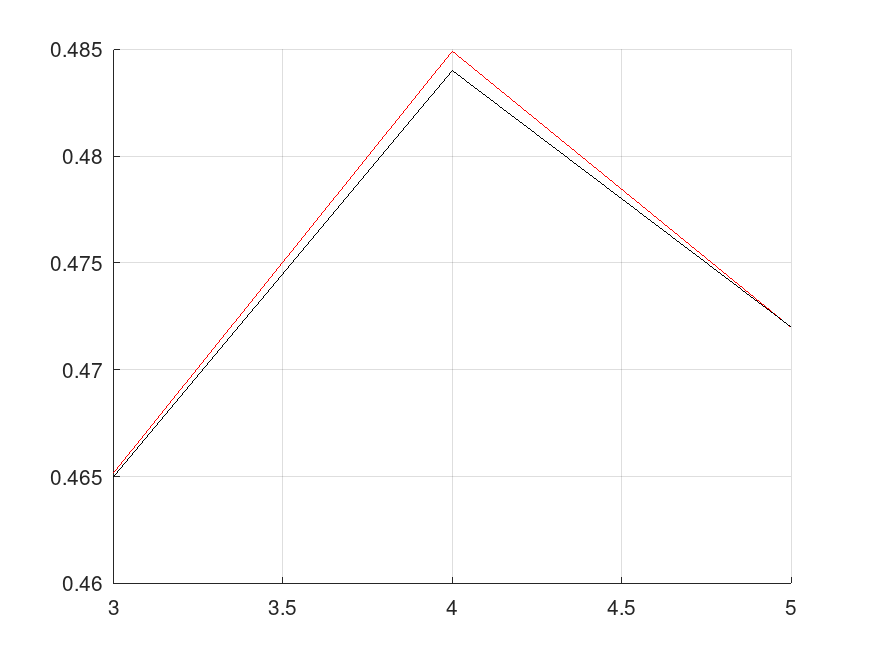
\includegraphics[width=0.8\textwidth]{images/task_5.png}
\end{figure}

Теперь найдем погрешность $|R_{2}(x)|$:\\[2mm]
\begin{align*}
  |R_{2}(x)| &= \frac{f^{(3)}(x)}{3!}(x-x_{0})(x-x_{1})(x-x_{2}) \\[1mm]
  |R_{2}(x)| & \leq \frac{M_{3}}{3!}(x-x_{0})(x-x_{1})(x-x_{2}) \\[1mm]
  M_{3} &= \max_{\left[a, b\right]}|f^{(3)}(x)| \\[1mm]
  f^{(3)}(x) & = \frac{2}{x^{3}} - \frac{3}{8x^{2}\sqrt{2}}
\end{align*}
Максимум $f^{(3)}(x)$ на отрезке $[3, 5]$, достигается в точке $3$.
\begin{gather*}
  f^{(3)}(x) = 0.05 \\[1mm]
  |R_{2}(x)| \leq \frac{0.05}{6}(x-3)(x-4)(x-5) \leq \frac{1}{120}x^{3} - \frac{1}{10}x^{2} + \frac{47}{120}x - \frac{1}{2}
\end{gather*}
\section{Шестое задание}

\paragraph{Текст задания} ~\\
Заданную функцию будут интерполировать на отрезке $\left[a, b\right]$ по чебышёвским узлам с заданной точностью $|R_{n}(x) < \epsilon|$. Требуется (а) определить требуемое для заданной точности $\epsilon$ количество узлов (т.е. степеньинтерполяционного многочлена плюс 1) и (б) вычислить значения всех узлов и отметить их на действительной оси $Ox$ (если узлов окажется много, ограничиться вычислением значений наименьших 10 узлов).\\[3mm]
\[
  f(x) = x^{2} - \sin\left(\frac{x}{2}\right), \text{на отрезке} \left[\frac{\pi}{4}, \pi\right] \text{с точностью} \epsilon = 10^{-3}
\]
